%%%%%%%%%%%%%%%%%%%%%%%%%%%%%%%%%%%%%%%%%%%%%%%%%%%%%%%%%%%%%%%%%%
%%%%%%%% ICML 2014 EXAMPLE LATEX SUBMISSION FILE %%%%%%%%%%%%%%%%%
%%%%%%%%%%%%%%%%%%%%%%%%%%%%%%%%%%%%%%%%%%%%%%%%%%%%%%%%%%%%%%%%%%

% Use the following line _only_ if you're still using LaTeX 2.09.
%\documentstyle[icml2014,epsf,natbib]{article}
% If you rely on Latex2e packages, like most moden people use this:
\documentclass{article}

\usepackage{amsmath,amsthm}


% use Times
\usepackage{times}
% For figures
\usepackage{graphicx} % more modern
%\usepackage{epsfig} % less modern
\usepackage{subfigure} 

% For citations
\usepackage{natbib}

% For algorithms
\usepackage{algorithm}
\usepackage{algorithmic-kr}

% As of 2011, we use the hyperref package to produce hyperlinks in the
% resulting PDF.  If this breaks your system, please commend out the
% following usepackage line and replace \usepackage{icml2014} with
% \usepackage[nohyperref]{icml2014} above.
\usepackage{hyperref}


% Packages hyperref and algorithmic misbehave sometimes.  We can fix
% this with the following command.
\newcommand{\theHalgorithm}{\arabic{algorithm}}







\usepackage{enumerate}





% Employ the following version of the ``usepackage'' statement for
% submitting the draft version of the paper for review.  This will set
% the note in the first column to ``Under review.  Do not distribute.''
%\usepackage{icml2014} 
% Employ this version of the ``usepackage'' statement after the paper has
% been accepted, when creating the final version.  This will set the
% note in the first column to ``Proceedings of the...''
\usepackage[accepted]{mynotes}

\newcommand{\argmax}{\texttt{argmax} }
\newcommand{\nn}{\nonumber }
\newcommand{\nnp}{\nonumber \\ }
\newcommand{\ie}{{\it i.e., }}
\newcommand{\expct}{\mathbf E}
\newcommand{\bp}{{\bf p }}
\newcommand{\bV}{{\bf V }}
\newcommand{\bff}{{\bf f }}
\newcommand{\bpt}{{\bf \hat{p} }}
\newtheorem{theorem}{Theorem}
\newtheorem{lemma}[theorem]{Lemma}
\newcommand{\BlackBox}{\rule{1.5ex}{1.5ex}}  % end of proof
\renewenvironment{proof}{\par\noindent{\bf Proof\ }}{\hfill\BlackBox\\[2mm]}

%\theoremstyle{definition}
\newtheorem{defn}{Definition}

% The \icmltitle you define below is probably too long as a header.
% Therefore, a short form for the running title is supplied here:
\icmltitlerunning{Predicting Venture Capital Investments}

\begin{document} 

\twocolumn[
\icmltitle{VCPredict: A Predictive Model of Venture Capital Investments}

% It is OKAY to include author information, even for blind
% submissions: the style file will automatically remove it for you
% unless you've provided the [accepted] option to the icml2014
% package.
\icmlauthor{Akilesh Potti}{avp39@cornell.edu}
%\icmladdress{Cornell Venture Capital}
\icmlauthor{Siddharth Reddy}{sgr45@cornell.edu}
%\icmladdress{Cornell Venture Capital}

% You may provide any keywords that you 
% find helpful for describing your paper; these are used to populate 
% the "keywords" metadata in the PDF but will not be shown in the document
\icmlkeywords{venture capital, machine learning}

\vskip 0.3in
]

\begin{abstract}
Venture capital firms are a major source of funding to start-up companies that would otherwise be unattractive investments to traditional investors and financial institutions. A wealth of public data is available about start-ups and VC firms through platforms like Crunchbase and AngelList. These data are useful for understanding the underlying structure of the venture capital space. We develop a predictive model of venture capital investments using various characteristics of start-up companies and VC firms, motivated by the following possible applications: (1) optimizing the fundraising process for start-up companies, and (2) optimizing the investment process for VC firms. As a result of our analysis, we find that 
\end{abstract}

\vspace{-0.3in}

\section{Introduction}

\subsection{Motivation}
The goal of our analysis is to create a predictive model of venture capital investments, specifically our model will predict whether or not a venture capital firm will invest in a start-up company, and if so, the specific dollar amount. Start-up companies could use this model to optimize their efforts in search of VC funding; rather than seek investment from VC firms unlikely to invest in companies with their characteristics, they could focus their time on VC firms that are active in their industry, geographic region, or problem space. VC firms could use this model to optimize their search for new start-up companies to add to their portfolios, and to develop data-driven characterizations of their investment philosophies to use as marketing tools.

\section{Problem Setup}
We use unsupervised learning methods to discover structure in the Crunchbase data set, then use those results to construct a feature set for the following supervised learning tasks:

\begin{itemize}
\item{Prediction of whether or not a venture capital firm will make future investments in a start-up company}
\item{Conditional on the outcome of the previous task, prediction of the dollar amount invested}
\end{itemize}

\section{Data Sources}

\begin{itemize}
\item{Crunchbase: \verb+http://www.crunchbase.com/+\footnote{http://info.crunchbase.com/about/crunchbase-data-exports/}}
\item{AngelList: \verb+https://angel.co+\\}
\end{itemize}
We use a combination of datasets as no one dataset truly captures all of the pertinent information for making the analysis. Crunchbase is our primary source, with over 80,000 data points and 13 features. AngelList offers start-up data regarding founders, board members, employees, etc. that the Crunchbase data set lacks.

\section{General Approach}
In our unsupervised learning phase, we cluster VCs by average investment size, targeted industries, and investment stage using heuristic-based clustering methods.

For our prediction of binary VC investments (i.e. will a VC invest in this start-up?), we use a logistic regression model. 

For our prediction of specific dollar amounts invested by VCs, we use multiple linear regression and a regression tree model. 

\section{Methods}

\section{Unsupervised Learning Tasks}

We expect inherent structure in the diversity of VC firms. Some firms are early-stage, seed funds that invest primarily in young start-ups. Others are mid-stage, late-stage, tend to make large investments (>40 million USD), tend to make small investments (<10 million USD), etc. In order to characterize this structure according to available data fields such as number of Series A rounds made, number of private equity investments made, and average investment size, we apply the k-means clustering algorithm to the VC firms represented in the Crunchbase data set. Prior knowledge suggests the existence of three major clusters of firms, so we set K=3 and produce the following clusters.

Characteristics of VC firms such as distribution of investments across various funding rounds, geographic regions, and start-up industries are typically correlated. As such, we expect variation in VC firms to be characterized by relatively few factors. Principal component analysis of the VC firms represented in Crunchbase reveals two main principal components that account for much of the variation in VCs.

In practice, certain VC firms tend to invest in the same start-up companies as a result of similar interests, investment strategies, domain expertise, etc. The graph is defined as follows: VC firms are represented as nodes, and edges are drawn between VC firms with weights proportional to the number of companies they have invested in together. The following ranking of VC firms is constructed using various graph centrality measures. A simple web page has also been setup to allow users to explore the co-investment graph.

\section{Supervised Learning Tasks}

In our prediction of binary VC investments, we use the following feature set:
\begin{itemize}
\item{Age (days)}
\item{Total funds raised to date (USD)}
\item{Binarized company industry (e.g. biotech, ecommerce)}
\item{Binarized company location (country)}
\item{Binarized types of past investors (e.g. has received investments from early-stage, mid-stage, and/or late-stage funds)}
\item{Average centrality of founders, advisors, board members, current and past investors in the co-investment graph}
\item{Number of employees}
\end{itemize}





\section{Results}

\subsection{Clustering}

% Table created by stargazer v.5.0 by Marek Hlavac, Harvard University. E-mail: hlavac at fas.harvard.edu
% Date and time: Mon, May 12, 2014 - 00:32:07
\begin{table}[!htbp] \centering 
  \caption{Centers produced by k-means clustering of VC firms.} 
  \label{VC Cluster Centers} 
\begin{tabular}{@{\extracolsep{5pt}} cccc} 
\\[-1.8ex]\hline 
\hline \\[-1.8ex] 
 & Late-stage & Mid-stage & Early-stage \\ 
angel & $0.017$ & $0.023$ & $0.324$ \\ 
crowdfunding & $0$ & $0.0001$ & $0.0001$ \\ 
other & $0$ & $0.012$ & $0.005$ \\ 
post.ipo & $0.008$ & $$-$0$ & $0$ \\ 
private.equity & $0.842$ & $0.012$ & $0.004$ \\ 
series.a & $0.067$ & $0.194$ & $0.449$ \\ 
series.b & $0.042$ & $0.214$ & $0.075$ \\ 
series.c. & $0.017$ & $0.253$ & $0.031$ \\ 
venture & $0.008$ & $0.293$ & $0.112$ \\ 
total & $4.170$ & $59.500$ & $26.800$ \\ 
\hline \\[-1.8ex] 
\end{tabular} 
\end{table} 

\begin{figure}[ht]
\vskip 0.2in
\begin{center}
\centerline{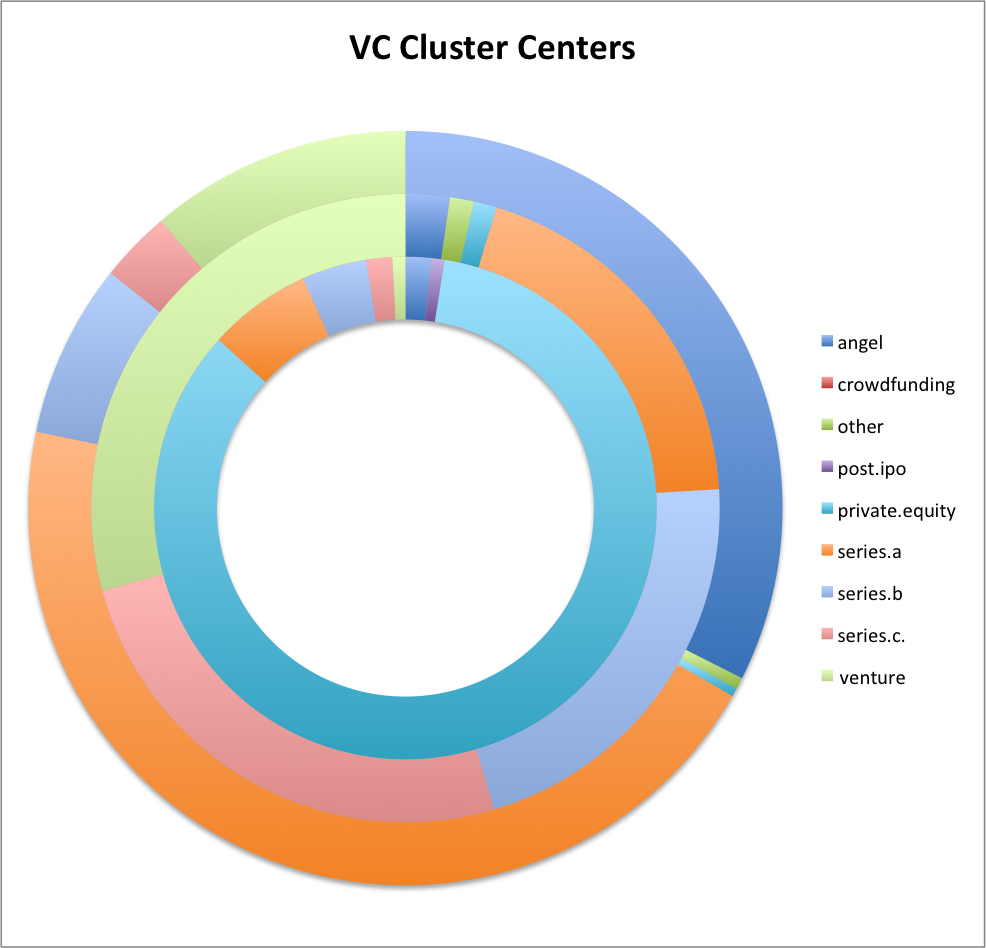
\includegraphics[width=\columnwidth]{cluster-centers.png}}
\caption{Centers produced by k-means clustering of VC firms. Outer ring, middle ring, and inner ring correspond to early-stage, mid-stage, and late-stage funds respectively.}
\label{VC Cluster Centers}
\end{center}
\vskip -0.2in
\end{figure}

\begin{figure}[ht]
\vskip 0.2in
\begin{center}
\centerline{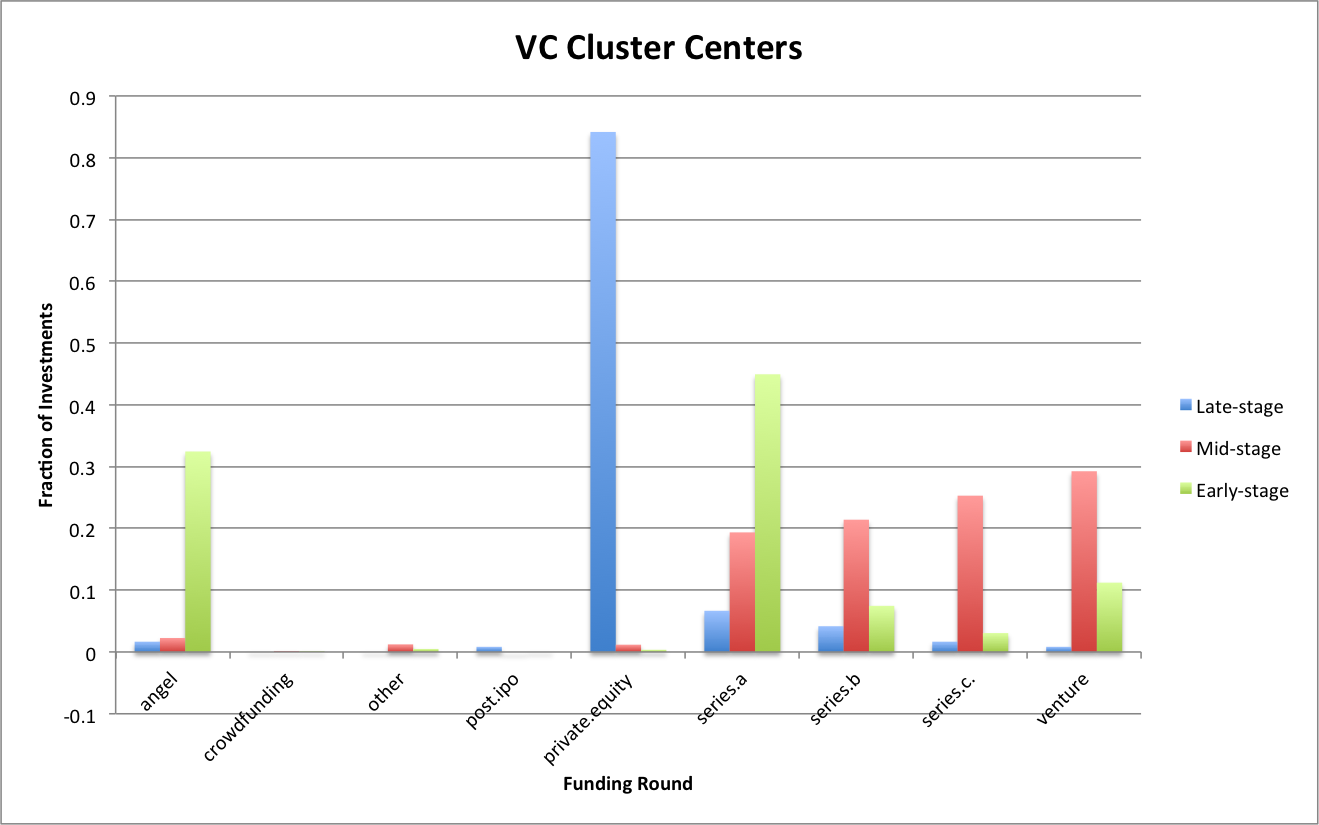
\includegraphics[width=\columnwidth]{cluster-centers-2.png}}
\caption{Centers produced by k-means clustering of VC firms.}
\label{VC Cluster Centers}
\end{center}
\vskip -0.2in
\end{figure}

\subsection{Principal Component Analysis}

% Table created by stargazer v.5.0 by Marek Hlavac, Harvard University. E-mail: hlavac at fas.harvard.edu
% Date and time: Mon, May 12, 2014 - 00:06:54
\begin{table}[!htbp] \centering 
  \caption{Importance of components} 
  \label{PCA of VC Investments} 
\begin{tabular}{@{\extracolsep{5pt}} cc} 
\\[-1.8ex]\hline 
\hline \\[-1.8ex] 
 & Proportion of Variance ($>0.01$) \\ 
Comp.1 & $0.861$ \\ 
Comp.2 & $0.075$ \\ 
Comp.3 & $0.042$ \\ 
\hline \\[-1.8ex] 
\end{tabular} 
\end{table} 

\begin{figure}[ht]
\vskip 0.2in
\begin{center}
\centerline{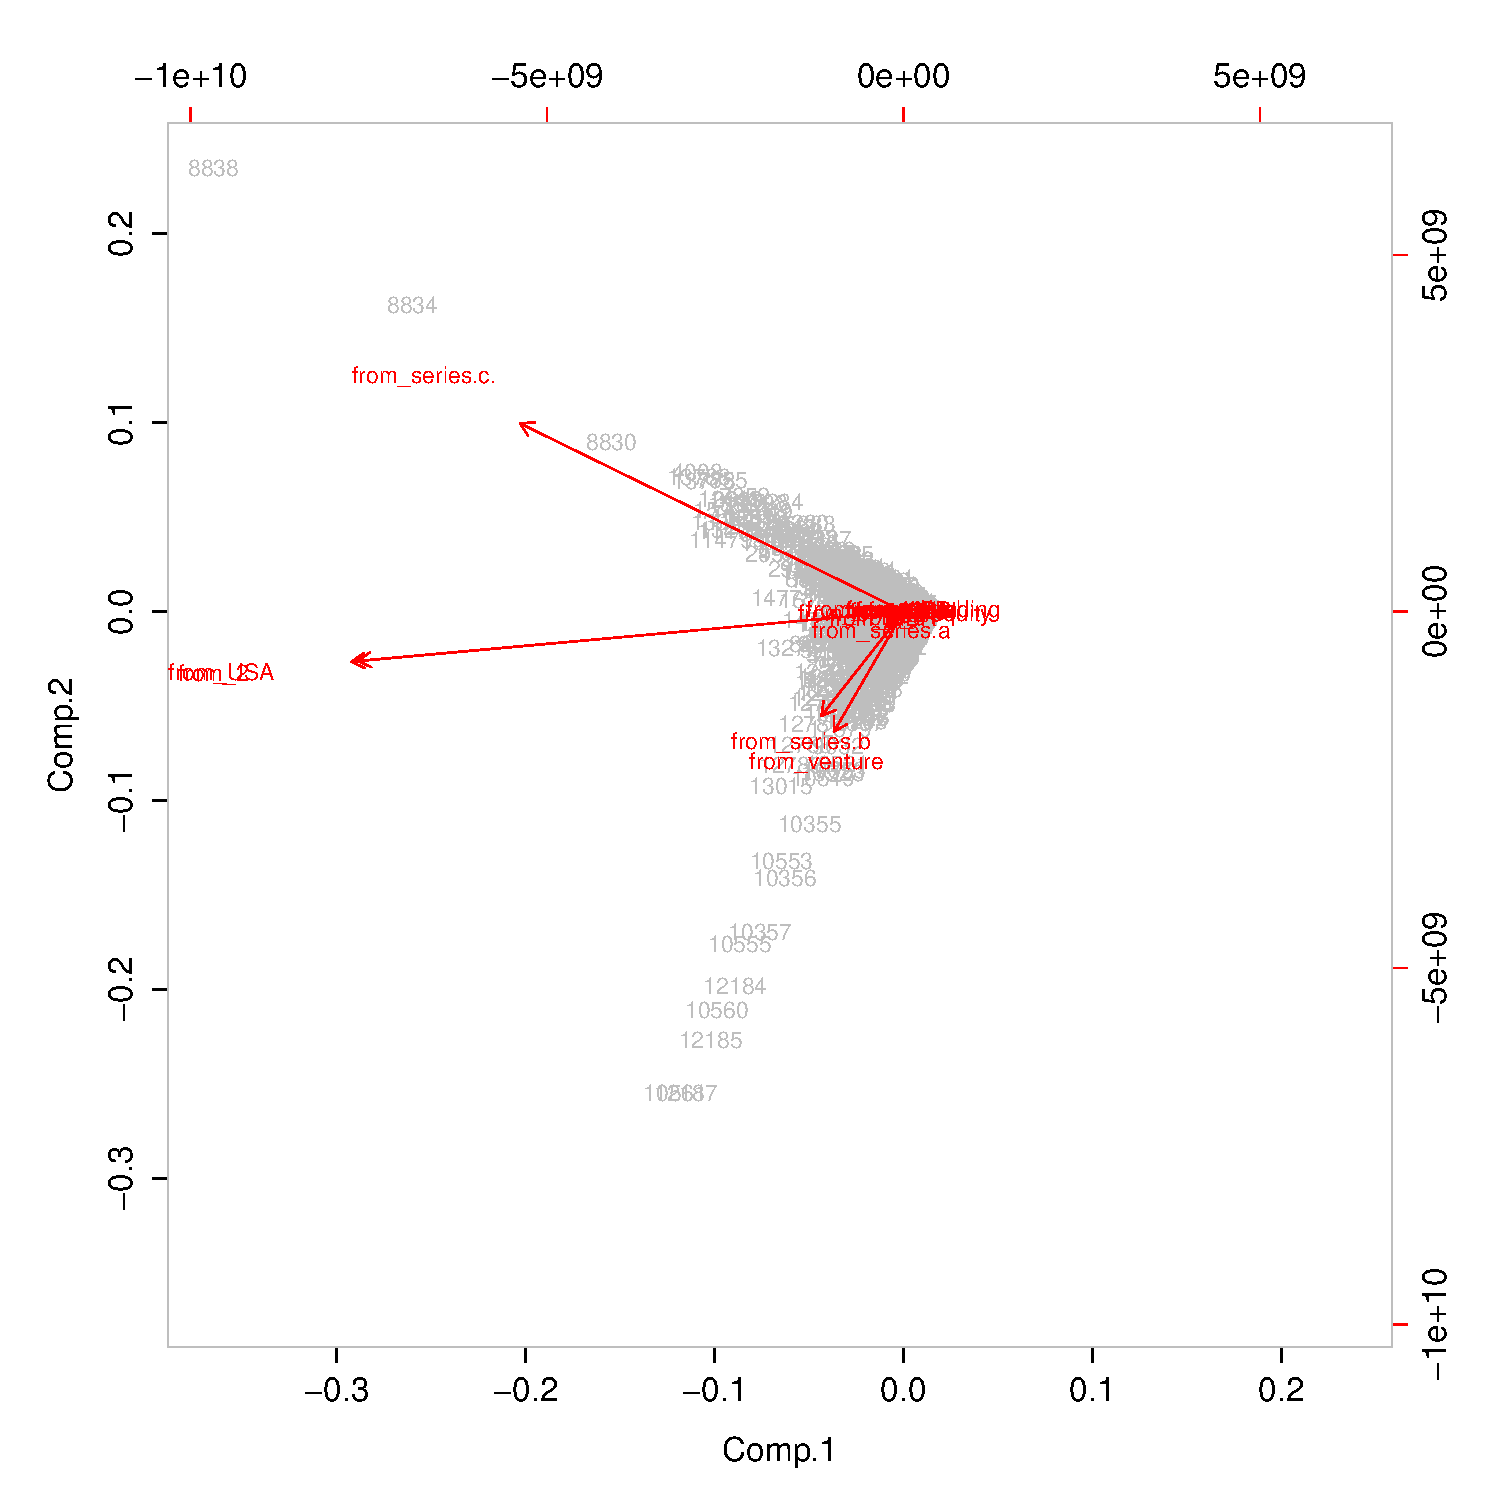
\includegraphics[width=\columnwidth]{pca-biplot.pdf}}
\caption{PCA of VC-Startup investments based on how much the start-up has raised from different types of VCs in the past, age, and total funds raised to date}
\label{PCA of VC Investments}
\end{center}
\vskip -0.2in
\end{figure}

% Table created by stargazer v.5.0 by Marek Hlavac, Harvard University. E-mail: hlavac at fas.harvard.edu
% Date and time: Mon, May 12, 2014 - 00:16:17
\begin{table}[!htbp] \centering 
  \caption{Importance of components} 
  \label{PCA of VC Firms} 
\begin{tabular}{@{\extracolsep{5pt}} cc} 
\\[-1.8ex]\hline 
\hline \\[-1.8ex] 
 & Proportion of Variance ($>0.1$) \\ 
Comp.1 & $0.362$ \\ 
Comp.2 & $0.276$ \\ 
Comp.3 & $0.184$ \\ 
Comp.4 & $0.117$ \\ 
\hline \\[-1.8ex] 
\end{tabular} 
\end{table} 

\begin{figure}[ht]
\vskip 0.2in
\begin{center}
\centerline{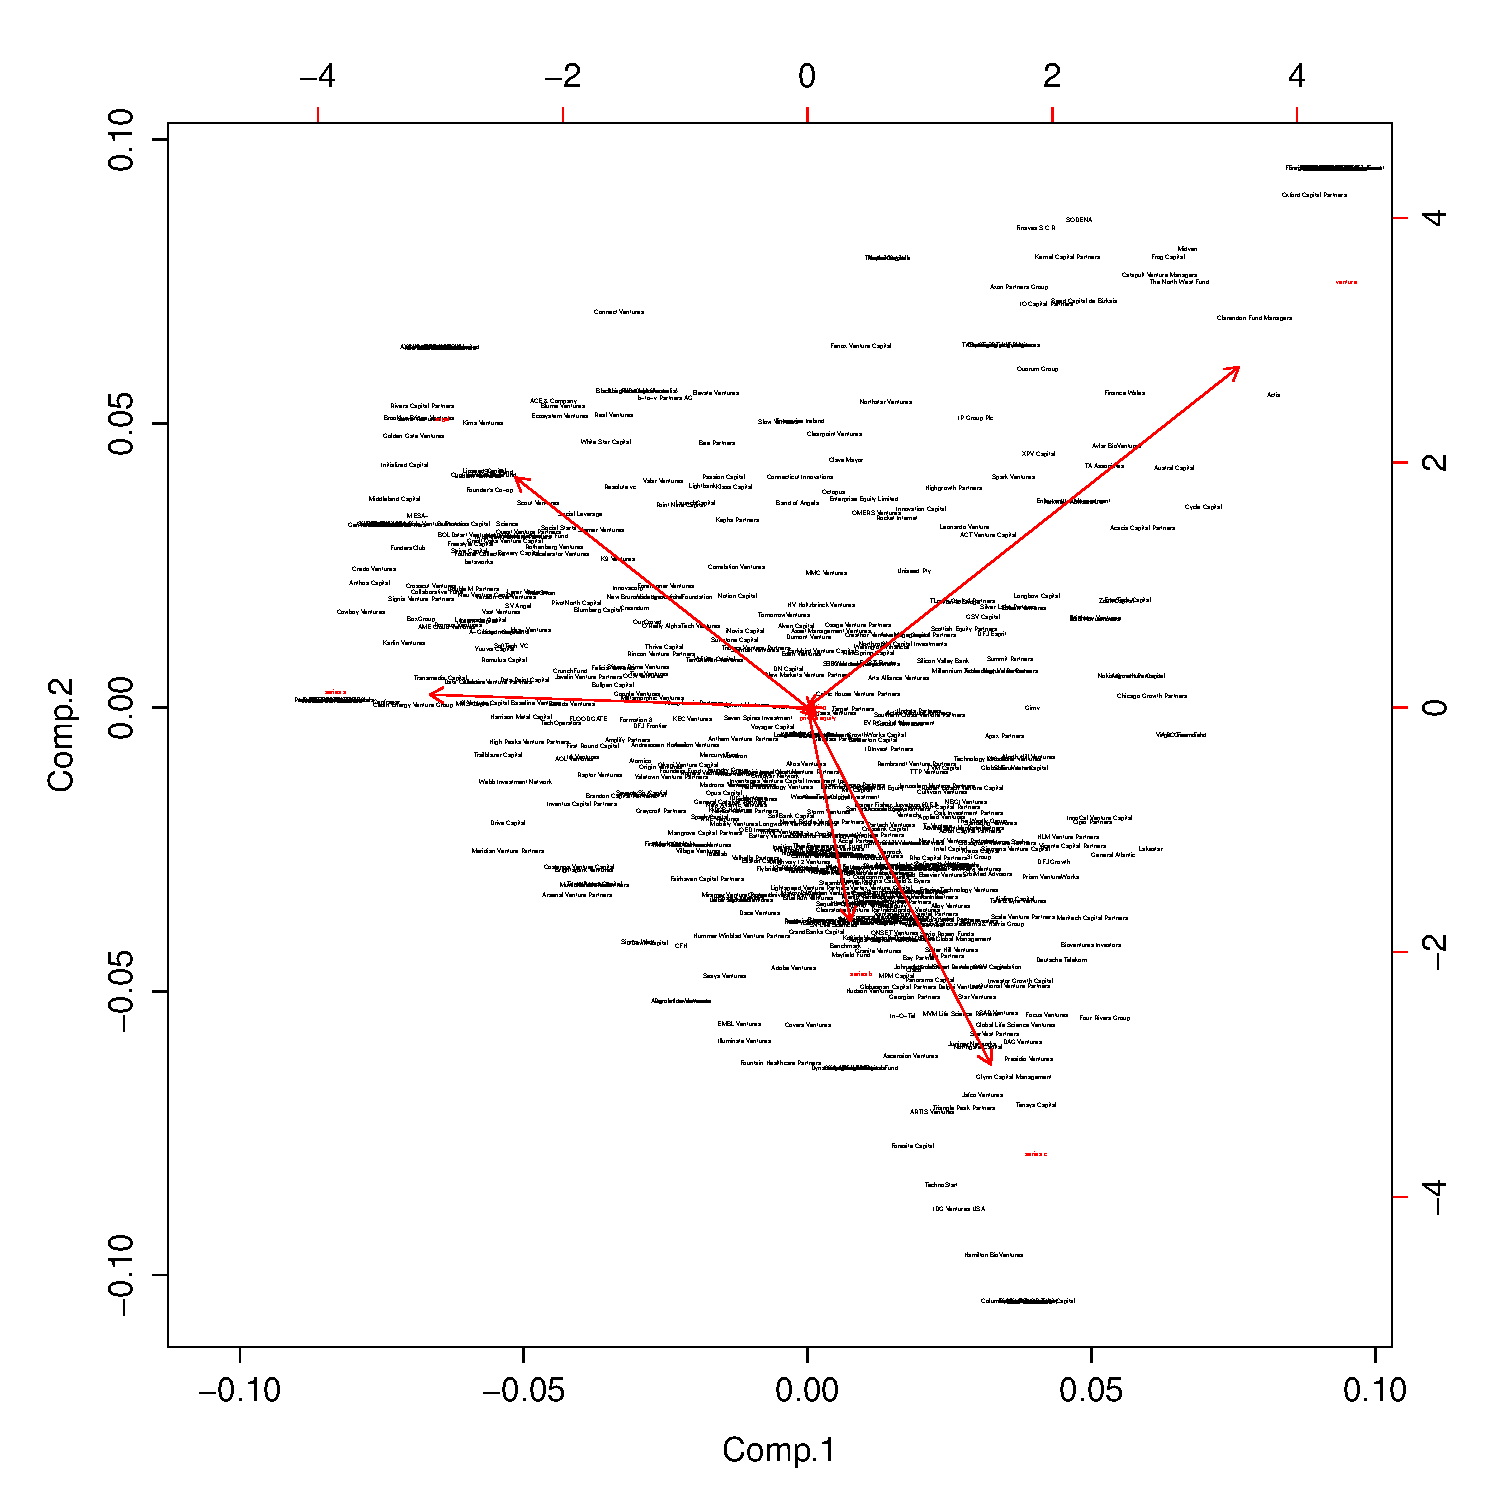
\includegraphics[width=\columnwidth]{pca-biplot-2.pdf}}
\caption{PCA of VC firms based on distribution of investments across different funding rounds (e.g. Series A/B/C, Angel)}
\label{PCA of VC Firms}
\end{center}
\vskip -0.2in
\end{figure}

\subsection{Co-investment Graph}

% Table created by stargazer v.5.0 by Marek Hlavac, Harvard University. E-mail: hlavac at fas.harvard.edu
% Date and time: Mon, May 12, 2014 - 01:10:05
\begin{table}[!htbp] \centering 
  \caption{Top 10 VC firms by Pagerank (eigenvector centrality) in the co-investment graph} 
  \label{Co-investment Centrality Ranking of VCs} 
\begin{tabular}{@{\extracolsep{5pt}} ccccccc} 
\\[-1.8ex]\hline 
\hline \\[-1.8ex] 
& Pagerank & In.degree.Centrality & Out.degree.Centrality & Closeness.Centrality & Betweenness.Centrality \\ 
SV Angel & $0.025$ & $0.385$ & $0.385$ & $0.541$ & $0.025$ \\ 
Intel Capital & $0.014$ & $0.395$ & $0.395$ & $0.554$ & $0.048$ \\ 
Accel Partners & $0.013$ & $0.359$ & $0.359$ & $0.536$ & $0.031$ \\ 
First Round Capital & $0.013$ & $0.306$ & $0.306$ & $0.504$ & $0.009$ \\ 
Kleiner Perkins Caufield \& Byers & $0.012$ & $0.332$ & $0.332$ & $0.522$ & $0.021$ \\ 
New Enterprise Associates & $0.012$ & $0.346$ & $0.346$ & $0.529$ & $0.022$ \\ 
Andreessen Horowitz & $0.011$ & $0.271$ & $0.271$ & $0.492$ & $0.008$ \\ 
Draper Fisher Jurvetson (DFJ) & $0.011$ & $0.346$ & $0.346$ & $0.530$ & $0.027$ \\ 
Sequoia Capital & $0.010$ & $0.281$ & $0.281$ & $0.503$ & $0.011$ \\ 
Greylock Partners & $0.010$ & $0.294$ & $0.294$ & $0.504$ & $0.010$ \\ 
\hline \\[-1.8ex] 
\end{tabular} 
\end{table}

\begin{figure}[ht]
\vskip 0.2in
\begin{center}
\centerline{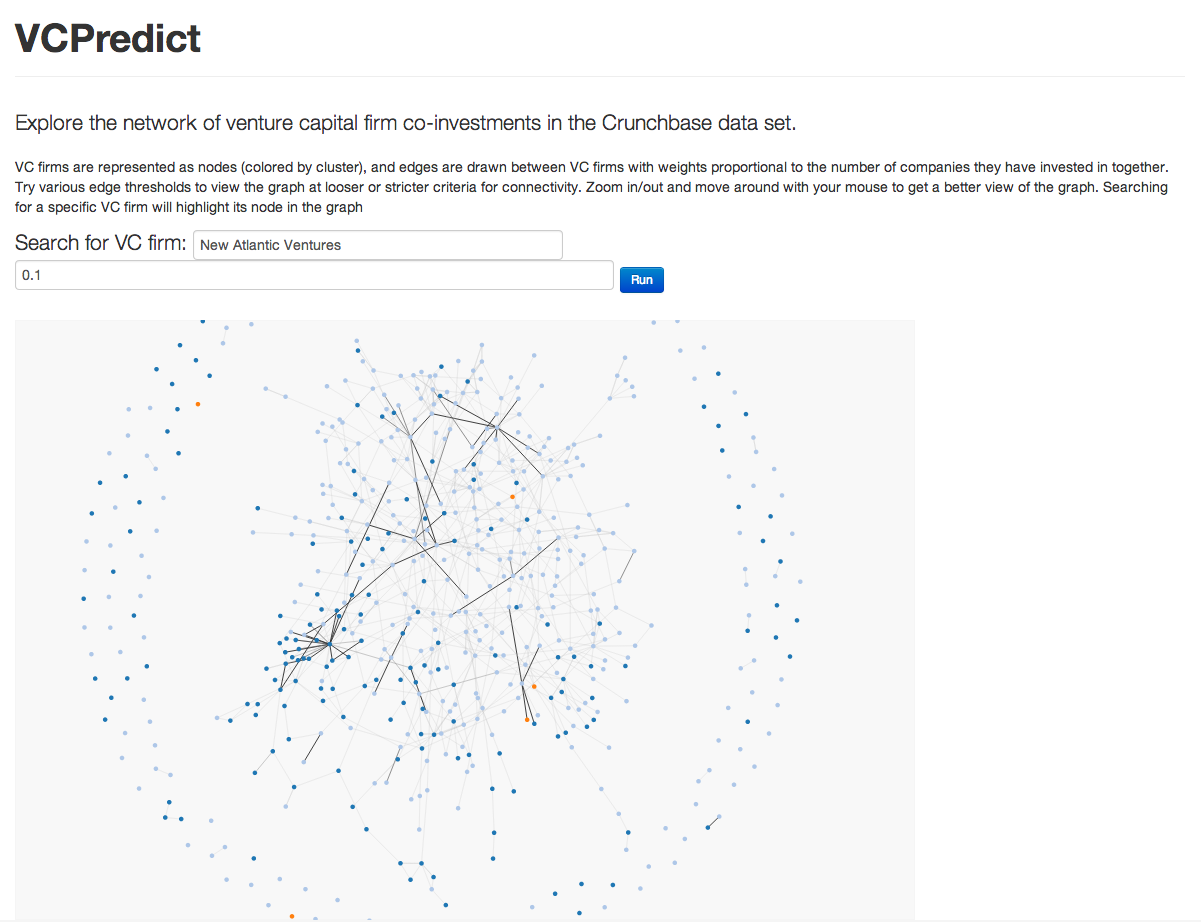
\includegraphics[width=\columnwidth]{vcpredict-web.png}}
\caption{Screenshot of interactive web page that allows users to explore the VC co-investment graph}
\label{Co-investment graph}
\end{center}
\vskip -0.2in
\end{figure}

\section{Conclusions}

\section{Bibliography}



\end{document} 



